\documentclass[]{article}
\usepackage{lmodern}
\usepackage{amssymb,amsmath}
\usepackage{ifxetex,ifluatex}
\usepackage{fixltx2e} % provides \textsubscript
\ifnum 0\ifxetex 1\fi\ifluatex 1\fi=0 % if pdftex
  \usepackage[T1]{fontenc}
  \usepackage[utf8]{inputenc}
\else % if luatex or xelatex
  \ifxetex
    \usepackage{mathspec}
  \else
    \usepackage{fontspec}
  \fi
  \defaultfontfeatures{Ligatures=TeX,Scale=MatchLowercase}
\fi
% use upquote if available, for straight quotes in verbatim environments
\IfFileExists{upquote.sty}{\usepackage{upquote}}{}
% use microtype if available
\IfFileExists{microtype.sty}{%
\usepackage{microtype}
\UseMicrotypeSet[protrusion]{basicmath} % disable protrusion for tt fonts
}{}
\usepackage[margin=1in]{geometry}
\usepackage{hyperref}
\hypersetup{unicode=true,
            pdftitle={Jackknife variance estimation corrections},
            pdfauthor={Xuelong Wang},
            pdfborder={0 0 0},
            breaklinks=true}
\urlstyle{same}  % don't use monospace font for urls
\usepackage{graphicx,grffile}
\makeatletter
\def\maxwidth{\ifdim\Gin@nat@width>\linewidth\linewidth\else\Gin@nat@width\fi}
\def\maxheight{\ifdim\Gin@nat@height>\textheight\textheight\else\Gin@nat@height\fi}
\makeatother
% Scale images if necessary, so that they will not overflow the page
% margins by default, and it is still possible to overwrite the defaults
% using explicit options in \includegraphics[width, height, ...]{}
\setkeys{Gin}{width=\maxwidth,height=\maxheight,keepaspectratio}
\IfFileExists{parskip.sty}{%
\usepackage{parskip}
}{% else
\setlength{\parindent}{0pt}
\setlength{\parskip}{6pt plus 2pt minus 1pt}
}
\setlength{\emergencystretch}{3em}  % prevent overfull lines
\providecommand{\tightlist}{%
  \setlength{\itemsep}{0pt}\setlength{\parskip}{0pt}}
\setcounter{secnumdepth}{5}
% Redefines (sub)paragraphs to behave more like sections
\ifx\paragraph\undefined\else
\let\oldparagraph\paragraph
\renewcommand{\paragraph}[1]{\oldparagraph{#1}\mbox{}}
\fi
\ifx\subparagraph\undefined\else
\let\oldsubparagraph\subparagraph
\renewcommand{\subparagraph}[1]{\oldsubparagraph{#1}\mbox{}}
\fi

%%% Use protect on footnotes to avoid problems with footnotes in titles
\let\rmarkdownfootnote\footnote%
\def\footnote{\protect\rmarkdownfootnote}

%%% Change title format to be more compact
\usepackage{titling}

% Create subtitle command for use in maketitle
\providecommand{\subtitle}[1]{
  \posttitle{
    \begin{center}\large#1\end{center}
    }
}

\setlength{\droptitle}{-2em}

  \title{Jackknife variance estimation corrections}
    \pretitle{\vspace{\droptitle}\centering\huge}
  \posttitle{\par}
    \author{Xuelong Wang}
    \preauthor{\centering\large\emph}
  \postauthor{\par}
      \predate{\centering\large\emph}
  \postdate{\par}
    \date{2019-12-12}

\usepackage{booktabs}
\usepackage{longtable}
\usepackage{array}
\usepackage{multirow}
\usepackage[table]{xcolor}
\usepackage{wrapfig}
\usepackage{float}
\usepackage{colortbl}
\usepackage{pdflscape}
\usepackage{tabu}
\usepackage{threeparttable}
\usepackage{threeparttablex}
\usepackage[normalem]{ulem}
\usepackage{makecell}

\usepackage{float,amsmath, bbm, amssymb, siunitx, bm}
\usepackage{pdfpages}
\floatplacement{figure}{H}
\newcommand{\indep}{\rotatebox[origin=c]{90}{$\models$}}

\begin{document}
\maketitle

{
\setcounter{tocdepth}{2}
\tableofcontents
}
\section{Jackknife variance
correction}\label{jackknife-variance-correction}

If we assume the \(S\) is a smooth functions of emperical CDF,
especially a quadratic functions, then it can be shown the leading terms
of
\(E(\tilde{Var}(S(X_1, \dots, S_{n-1}))) \geq Var(S(X_1, \dots, S_{n-1}))\)
is a quadratic term in expecation. Therefore we could try to estimate
the quadratic term and correct the bias for the jackknife variance
estimation.

Define \(Q_{ii'} \equiv nS - (n-1)(S_{i} + S_{i'}) + (n-2)S_{(ii')}\),
then the correction will be \[
\hat{Var}^{corr}(S(X_1, \dots, X_n)) = \hat{Var}(S(X_1, \dots, X_n)) - \frac{1}{n(n-1)}\sum_{i < i'}(Q_{ii'}- \bar{Q})^2
\] where \(\bar{Q} = \sum_{i < i'}(Q_{ii'})/(n(n-1)/2)\)

\section{Simulation study compare two GCTA and
GCTA\_rr}\label{simulation-study-compare-two-gcta-and-gcta_rr}

GCTA\_rr is the \texttt{mixed.solve} function from \texttt{rrBLUP} r
package.\\
Based on the following simulation results,

\begin{enumerate}
\def\labelenumi{\arabic{enumi}.}
\tightlist
\item
  when \(n<p\) case, those two methods' results are very closed to each
  other.
\item
  when \(n>p\) case, in terms of effect estimation and jackknife
  variance estimation those two methods's reuslts are similar to each
  other. But for the variance corrections are quite different. That is
  the statistics \(Q\) of our method has a very large variance which
  leads to negative correction result.
\end{enumerate}

\subsubsection{setup}\label{setup}

\begin{itemize}
\tightlist
\item
  Independent
\item
  Normal
\item
  \(p = 100\)
\item
  \(n = \{50, 75,100, 150, 200\}\)
\item
  with interaction terms
\item
  main effect: \(Var(X^T\beta) = \{0,8,100\}\) \newpage
\end{itemize}

\subsubsection{Simulation result}\label{simulation-result}

\subsubsection{\texorpdfstring{\(Var(X^T\beta) = \{0\}\)}{Var(X\^{}T\textbackslash{}beta) = \textbackslash{}\{0\textbackslash{}\}}}\label{varxtbeta-0}

\begin{verbatim}
     n  MSE est_var est_mean NA_main GCTA_main_jack GCTA_v_jack_1
1:  50 3.40    1.83     1.32       0           0.59          9.55
2:  75 1.19    0.98     0.56       0           0.46          2.73
3: 100 1.08    0.84     0.57       0           0.44          1.35
4: 150 0.28    0.19     0.32       0          -1.09          0.86
5: 200 0.21    0.12     0.32       0          -1.60          0.78
   GCTA_v_jack_2 GCTA_v_corr
1:          9.62       -9.28
2:          2.68       -5.64
3:          1.35       -0.77
4:          0.67      -64.08
5:          0.69      -46.14
\end{verbatim}

\begin{verbatim}
     n  MSE est_var est_mean NA_main GCTA_rr_main_jack GCTA_rr_v_jack_1
1:  50 3.40    1.83     1.32       0              0.60             9.55
2:  75 1.19    0.98     0.56       0              0.46             2.73
3: 100 1.08    0.84     0.57       0              0.44             1.35
4: 150 0.28    0.19     0.33       0             -0.17             0.62
5: 200 0.21    0.12     0.33       0              0.28             0.61
   GCTA_rr_v_jack_2 GCTA_rr_v_corr
1:             9.47         -3.560
2:             2.68         -5.643
3:             1.35         -0.770
4:             0.61         -1.204
5:             0.61         -0.041
\end{verbatim}

\subsubsection{\texorpdfstring{\(Var(X^T\beta) = \{100\}\)}{Var(X\^{}T\textbackslash{}beta) = \textbackslash{}\{100\textbackslash{}\}}}\label{varxtbeta-100}

\begin{verbatim}
     n   MSE est_var est_mean NA_main GCTA_main_jack GCTA_v_jack_1
1:  50  9247    1784       87       0             66          8795
2:  75 10077    1863       92       0            103          5170
3: 100 11839    2142      100       0             84          2072
4: 150 10953     443      103       0             31          1280
5: 200  9778     245       98       0             30           725
   GCTA_v_jack_2 GCTA_v_corr
1:          8793       -3687
2:          5109       -3122
3:          2081         194
4:          1148      -80475
5:           673      -32124
\end{verbatim}

\begin{verbatim}
     n   MSE est_var est_mean NA_main GCTA_rr_main_jack GCTA_rr_v_jack_1
1:  50  9247    1784       87       0                66             8795
2:  75 10077    1863       92       0               103             5170
3: 100 11839    2142      100       0                84             2072
4: 150 11194     414      104       0               103              969
5: 200  9854     238       98       0                98              616
   GCTA_rr_v_jack_2 GCTA_rr_v_corr
1:             8787          -3492
2:             5109          -3124
3:             2081            194
4:              970            158
5:              616            220
\end{verbatim}

\subsubsection{\texorpdfstring{\(Var(X^T\beta) = \{8\}\)}{Var(X\^{}T\textbackslash{}beta) = \textbackslash{}\{8\textbackslash{}\}}}\label{varxtbeta-8}

\begin{verbatim}
     n MSE est_var est_mean NA_main GCTA_main_jack GCTA_v_jack_1
1:  50  90    25.8      8.0       0            8.5          74.1
2:  75  70    13.1      7.5       0            7.5          32.1
3: 100  68     6.3      7.8       0            7.5          13.7
4: 150  70     4.0      8.1       0            8.4           9.2
5: 200  65     2.5      7.9       0            7.6           4.6
   GCTA_v_jack_2 GCTA_v_corr
1:          73.8     -190.67
2:          31.9      -25.67
3:          13.8       -0.97
4:           8.1     -502.59
5:           4.3     -214.51
\end{verbatim}

\begin{verbatim}
     n  MSE est_var est_mean NA_main
1:  50 24.0    24.0      8.0       0
2:  75 13.8    13.8      7.9       0
3: 100  8.6     8.6      8.1       0
4: 150  3.7     3.7      8.0       0
5: 200  2.7     2.7      8.0       0
\end{verbatim}

\begin{verbatim}
     n MSE est_var est_mean NA_main GCTA_rr_main_jack GCTA_rr_v_jack_1
1:  50  90    25.8      8.0       0               8.5             74.1
2:  75  70    13.1      7.5       0               7.5             32.1
3: 100  68     6.3      7.8       0               7.5             13.7
4: 150  70     4.1      8.1       0               8.1              6.9
5: 200  65     2.5      7.9       0               7.9              3.9
   GCTA_rr_v_jack_2 GCTA_rr_v_corr
1:             73.6        -177.35
2:             31.8         -16.78
3:             13.8          -0.97
4:              6.9           1.49
5:              3.9           1.38
\end{verbatim}

\begin{verbatim}
     n  MSE est_var est_mean NA_main
1:  50 23.8    23.9      8.0       0
2:  75 13.7    13.7      7.9       0
3: 100  8.6     8.6      8.1       0
4: 150  3.8     3.8      8.0       0
5: 200  2.7     2.7      8.1       0
\end{verbatim}

\subsubsection{correlation test \$}\label{correlation-test}

\begin{verbatim}
     n    MSE est_var est_mean NA_main cor_main_jack cor_v_jack_1
1:  50 0.0131  0.0130     0.49       0          0.49       0.0127
2:  75 0.0083  0.0083     0.50       0          0.50       0.0079
3: 100 0.0057  0.0057     0.50       0          0.50       0.0059
4: 150 0.0038  0.0038     0.50       0          0.50       0.0039
5: 200 0.0030  0.0030     0.50       0          0.50       0.0029
   cor_v_jack_2 cor_v_corr
1:       0.0128     0.0120
2:       0.0079     0.0076
3:       0.0059     0.0057
4:       0.0039     0.0038
5:       0.0029     0.0029
\end{verbatim}

\subsection{compare the performance of delete 1 and delete d in variance
estimation}\label{compare-the-performance-of-delete-1-and-delete-d-in-variance-estimation}

The delete-d jackknife varinace estimator is \[
\mathcal{v}_{J(d)} = \frac{n-d}{d} \cdot \frac{1}{S}\sum_{S}(\hat{\theta}_s - \hat{\theta}_{s.} )
\], where \(S =\binom{n}{d}\). Note that S could a very large value, so
in the following simulation, only \(S = 1000\) is used. In Jun Shao's
another paper, he proposed an approximation of the deletel-d variance
estimation. That is just select m from \(S =\binom{n}{d}\) sub-samples
and in that paper it recommended \(m = n^{1.5}\).

\subsubsection{setup}\label{setup-1}

\begin{itemize}
\tightlist
\item
  Independent
\item
  Normal
\item
  \(p = \{100, 1000\}\)
\item
  \(n = \{50, 75,100, 150, 200, 500, 750,1000, 1500, 2000\}\)
\item
  \(d = 0.5 \times n\)
\item
  \(n_{repeat} = 1000\) for delete d jackknife
\item
  main effect: \(Var(X^T\beta) = 8\)
\end{itemize}

\newpage

\subsubsection{GCTA with p = 100}\label{gcta-with-p-100}

\begingroup\fontsize{7}{9}\selectfont

\begin{longtable}{rrrrrrrrrr}
\toprule
n & MSE & est\_var & est\_mean & NA\_main & GCTA\_main\_jack & GCTA\_v\_jack & GCTA\_v\_jack\_var & d & n\_sub\\
\midrule
\endfirsthead
\multicolumn{10}{@{}l}{\textit{(continued)}}\\
\toprule
n & MSE & est\_var & est\_mean & NA\_main & GCTA\_main\_jack & GCTA\_v\_jack & GCTA\_v\_jack\_var & d & n\_sub\\
\midrule
\endhead
\
\endfoot
\bottomrule
\endlastfoot
50 & 25.6 & 25.8 & 8.0 & 0 & 8.5 & 74.1 & 8383.8 & 1.0 & NA\\
75 & 13.2 & 13.1 & 7.5 & 0 & 7.5 & 32.1 & 685.1 & 1.0 & NA\\
100 & 6.2 & 6.3 & 7.8 & 0 & 7.5 & 13.7 & 102.2 & 1.0 & NA\\
150 & 4.0 & 4.0 & 8.1 & 0 & 8.4 & 9.2 & 16.4 & 1.0 & NA\\
200 & 2.5 & 2.5 & 7.9 & 0 & 7.6 & 4.6 & 2.1 & 1.0 & NA\\
\addlinespace
50 & 25.6 & 25.8 & 8.0 & 0 & 45.5 & 41.2 & 365.2 & 0.5 & NA\\
75 & 13.2 & 13.1 & 7.5 & 0 & -177.5 & 27.1 & 99.7 & 0.5 & NA\\
100 & 6.2 & 6.3 & 7.8 & 0 & -237.3 & 18.5 & 38.1 & 0.5 & NA\\
150 & 4.0 & 4.0 & 8.1 & 0 & -13.8 & 9.4 & 7.5 & 0.5 & NA\\
200 & 2.5 & 2.5 & 7.9 & 0 & 17.3 & 5.0 & 1.4 & 0.5 & NA\\
\addlinespace
50 & 25.6 & 25.8 & 8.0 & 0 & 35.1 & 41.1 & 366.6 & 0.5 & 354\\
75 & 13.2 & 13.1 & 7.5 & 0 & -107.6 & 27.0 & 100.1 & 0.5 & 650\\
100 & 6.2 & 6.3 & 7.8 & 0 & -237.3 & 18.5 & 38.1 & 0.5 & 1000\\
150 & 4.0 & 4.0 & 8.1 & 0 & -20.2 & 9.3 & 7.0 & 0.5 & 1837\\
200 & 2.5 & 2.5 & 7.9 & 0 & 53.4 & 5.1 & 1.3 & 0.5 & 2828\\*
\end{longtable}

\endgroup{}

\subsubsection{GCTA with p = 1000}\label{gcta-with-p-1000}

\begingroup\fontsize{7}{9}\selectfont

\begin{longtable}{rrrrrrrrr}
\toprule
n & MSE & est\_var & est\_mean & NA\_main & GCTA\_main\_jack & GCTA\_v\_jack & GCTA\_v\_jack\_var & d\\
\midrule
\endfirsthead
\multicolumn{9}{@{}l}{\textit{(continued)}}\\
\toprule
n & MSE & est\_var & est\_mean & NA\_main & GCTA\_main\_jack & GCTA\_v\_jack & GCTA\_v\_jack\_var & d\\
\midrule
\endhead
\
\endfoot
\bottomrule
\endlastfoot
500 & 2.88 & 2.91 & 8.0 & 0 & 7.8 & 4.65 & 1.08 & 1.0\\
750 & 1.29 & 1.30 & 8.0 & 0 & 8.0 & 2.26 & 0.15 & 1.0\\
1000 & 0.77 & 0.78 & 8.0 & 0 & 8.0 & 1.28 & 0.04 & 1.0\\
1500 & 0.47 & 0.48 & 7.9 & 0 & 6.7 & 0.80 & 0.01 & 1.0\\
500 & 2.88 & 2.91 & 8.0 & 0 & -79.1 & 6.56 & 1.17 & 0.5\\
\addlinespace
750 & 1.29 & 1.30 & 8.0 & 0 & -5.9 & 3.04 & 0.13 & 0.5\\
1000 & 0.77 & 0.78 & 8.0 & 0 & 40.8 & 1.71 & 0.05 & 0.5\\
1500 & 0.41 & 0.41 & 8.0 & 0 & 9.9 & 0.80 & 0.01 & 0.5\\
2000 & 0.31 & 0.31 & 8.0 & 0 & 25.6 & 0.48 & 0.00 & 0.5\\*
\end{longtable}

\endgroup{}

\subsubsection{GCTA\_rr\_rr with p = 100}\label{gcta_rr_rr-with-p-100}

\begingroup\fontsize{7}{9}\selectfont

\begin{longtable}{rrrrrrrrrr}
\toprule
n & MSE & est\_var & est\_mean & NA\_main & GCTA\_rr\_main\_jack & GCTA\_rr\_v\_jack & GCTA\_rr\_v\_jack\_var & d & n\_sub\\
\midrule
\endfirsthead
\multicolumn{10}{@{}l}{\textit{(continued)}}\\
\toprule
n & MSE & est\_var & est\_mean & NA\_main & GCTA\_rr\_main\_jack & GCTA\_rr\_v\_jack & GCTA\_rr\_v\_jack\_var & d & n\_sub\\
\midrule
\endhead
\
\endfoot
\bottomrule
\endlastfoot
50 & 25.6 & 25.8 & 8.0 & 0 & 8.5 & 74.1 & 8378.6 & 1.0 & NA\\
75 & 13.2 & 13.1 & 7.5 & 0 & 7.5 & 32.1 & 685.3 & 1.0 & NA\\
100 & 6.2 & 6.3 & 7.8 & 0 & 7.5 & 13.7 & 102.2 & 1.0 & NA\\
150 & 4.1 & 4.1 & 8.1 & 0 & 8.1 & 6.9 & 8.5 & 1.0 & NA\\
200 & 2.5 & 2.5 & 7.9 & 0 & 7.9 & 3.9 & 1.3 & 1.0 & NA\\
\addlinespace
50 & 25.6 & 25.8 & 8.0 & 0 & 52.5 & 40.6 & 363.1 & 0.5 & NA\\
75 & 13.2 & 13.1 & 7.5 & 0 & -198.0 & 26.6 & 100.2 & 0.5 & NA\\
100 & 6.2 & 6.3 & 7.8 & 0 & -257.6 & 18.1 & 38.6 & 0.5 & NA\\
150 & 4.1 & 4.1 & 8.1 & 0 & -11.9 & 9.3 & 7.5 & 0.5 & NA\\
200 & 2.5 & 2.5 & 7.9 & 0 & 25.4 & 5.0 & 1.4 & 0.5 & NA\\
\addlinespace
50 & 25.6 & 25.8 & 8.0 & 0 & 35.2 & 40.5 & 363.4 & 0.5 & 354\\
75 & 13.2 & 13.1 & 7.5 & 0 & -120.5 & 26.6 & 100.8 & 0.5 & 650\\
100 & 6.2 & 6.3 & 7.8 & 0 & -257.6 & 18.1 & 38.6 & 0.5 & 1000\\
150 & 4.1 & 4.1 & 8.1 & 0 & -17.0 & 9.3 & 7.1 & 0.5 & 1837\\
200 & 2.5 & 2.5 & 7.9 & 0 & 76.2 & 5.1 & 1.3 & 0.5 & 2828\\*
\end{longtable}

\endgroup{}

\subsubsection{GCTA\_rr with p = 1000}\label{gcta_rr-with-p-1000}

\begingroup\fontsize{7}{9}\selectfont

\begin{longtable}{rrrrrrrrr}
\toprule
n & MSE & est\_var & est\_mean & NA\_main & GCTA\_rr\_main\_jack & GCTA\_rr\_v\_jack & GCTA\_rr\_v\_jack\_var & d\\
\midrule
\endfirsthead
\multicolumn{9}{@{}l}{\textit{(continued)}}\\
\toprule
n & MSE & est\_var & est\_mean & NA\_main & GCTA\_rr\_main\_jack & GCTA\_rr\_v\_jack & GCTA\_rr\_v\_jack\_var & d\\
\midrule
\endhead
\
\endfoot
\bottomrule
\endlastfoot
500 & 2.88 & 2.91 & 8.0 & 0 & 7.8 & 4.65 & 1.08 & 1.0\\
750 & 1.29 & 1.30 & 8.0 & 0 & 8.0 & 2.26 & 0.15 & 1.0\\
1000 & 0.77 & 0.78 & 8.0 & 0 & 8.0 & 1.28 & 0.04 & 1.0\\
1500 & 0.48 & 0.48 & 7.9 & 0 & 8.0 & 0.62 & 0.00 & 1.0\\
500 & 2.88 & 2.91 & 8.0 & 0 & -79.1 & 6.56 & 1.17 & 0.5\\
\addlinespace
750 & 1.29 & 1.30 & 8.0 & 0 & -5.9 & 3.04 & 0.13 & 0.5\\
1000 & 0.77 & 0.78 & 8.0 & 0 & 40.8 & 1.71 & 0.05 & 0.5\\
1500 & 0.41 & 0.41 & 8.0 & 0 & 11.8 & 0.80 & 0.01 & 0.5\\
2000 & 0.31 & 0.31 & 8.0 & 0 & 24.4 & 0.48 & 0.00 & 0.5\\*
\end{longtable}

\endgroup{}

\subsubsection{cor with n = 200}\label{cor-with-n-200}

\begingroup\fontsize{7}{9}\selectfont

\begin{longtable}{rrrrrrrr}
\toprule
n & MSE & est\_var & est\_mean & NA\_main & cor\_main\_jack & cor\_v\_jack & d\\
\midrule
\endfirsthead
\multicolumn{8}{@{}l}{\textit{(continued)}}\\
\toprule
n & MSE & est\_var & est\_mean & NA\_main & cor\_main\_jack & cor\_v\_jack & d\\
\midrule
\endhead
\
\endfoot
\bottomrule
\endlastfoot
50 & 0.01252 & 0.01265 & 0.50001 & 0 & 0.50432 & 0.01229 & 1.0\\
75 & 0.00774 & 0.00782 & 0.50050 & 0 & 0.50323 & 0.00815 & 1.0\\
100 & 0.00607 & 0.00613 & 0.50148 & 0 & 0.50334 & 0.00582 & 1.0\\
150 & 0.00383 & 0.00385 & 0.49584 & 0 & 0.49709 & 0.00391 & 1.0\\
200 & 0.00281 & 0.00284 & 0.49930 & 0 & 0.50027 & 0.00288 & 1.0\\
\addlinespace
50 & 0.01252 & 0.01265 & 0.50001 & 0 & 5.32154 & 0.01282 & 0.5\\
75 & 0.00774 & 0.00782 & 0.50050 & 0 & 3.26213 & 0.00844 & 0.5\\
100 & 0.00607 & 0.00613 & 0.50148 & 0 & 2.50378 & 0.00595 & 0.5\\
150 & 0.00383 & 0.00385 & 0.49584 & 0 & 1.59064 & 0.00396 & 0.5\\
200 & 0.00281 & 0.00284 & 0.49930 & 0 & 1.46439 & 0.00293 & 0.5\\*
\end{longtable}

\endgroup{}

\subsubsection{median with n = 200}\label{median-with-n-200}

\begingroup\fontsize{7}{9}\selectfont

\begin{longtable}{rrrrrrrr}
\toprule
n & MSE & est\_var & est\_mean & NA\_main & median\_main\_jack & median\_v\_jack & d\\
\midrule
\endfirsthead
\multicolumn{8}{@{}l}{\textit{(continued)}}\\
\toprule
n & MSE & est\_var & est\_mean & NA\_main & median\_main\_jack & median\_v\_jack & d\\
\midrule
\endhead
\
\endfoot
\bottomrule
\endlastfoot
50 & 0.03138 & 0.03135 & -0.00775 & 0 & -0.00775 & 0.06818 & 1.0\\
75 & 0.02211 & 0.02212 & -0.00212 & 0 & 0.05228 & 0.03113 & 1.0\\
100 & 0.01523 & 0.01523 & -0.00378 & 0 & -0.00378 & 0.02720 & 1.0\\
150 & 0.01072 & 0.01072 & -0.00279 & 0 & -0.00279 & 0.01885 & 1.0\\
200 & 0.00804 & 0.00804 & -0.00051 & 0 & -0.00051 & 0.01614 & 1.0\\
\addlinespace
50 & 0.03138 & 0.03135 & -0.00775 & 0 & 5.04459 & 0.03477 & 0.5\\
75 & 0.02211 & 0.02212 & -0.00212 & 0 & 8.44376 & 0.02248 & 0.5\\
100 & 0.01523 & 0.01523 & -0.00378 & 0 & 2.68868 & 0.01587 & 0.5\\
150 & 0.01072 & 0.01072 & -0.00279 & 0 & -1.47581 & 0.01110 & 0.5\\
200 & 0.00804 & 0.00804 & -0.00051 & 0 & 3.96797 & 0.00827 & 0.5\\*
\end{longtable}

\endgroup{}

\subsection{Jackknife variance estimation's bias and sample size
n}\label{jackknife-variance-estimations-bias-and-sample-size-n}

\subsubsection{setup}\label{setup-2}

\begin{itemize}
\tightlist
\item
  Independent
\item
  Normal
\item
  \(p = 100\)
\item
  \(n = \{50, 75,100, 150, 200, 500, 750,1000, 1500, 2000\}\)
\item
  \(d = 0.5 \times n\)
\item
  \(n_{repeat} = n^{1.5}\) for delete d jackknife
\item
  main effect: \(Var(X^T\beta) = 8\)
\end{itemize}

Based on the previous simulation results, we find there is a bias among
all the jackknife variance estimation. Based on the Efron's result, the
overestimation is because the statistics \(S\) is not a smooth function
of the distribution function, so that the correct coefficient actually
inflate the variance estimation.

The following reuslt is trying to see the relation between the bias and
the sample size n

\subsubsection{GCTA with p = 100}\label{gcta-with-p-100-1}

\begingroup\fontsize{5}{7}\selectfont

\begin{longtable}{rrrrrrrrrr}
\toprule
n & MSE & est\_var & est\_mean & NA\_main & GCTA\_rr\_main\_jack & GCTA\_rr\_v\_jack & GCTA\_rr\_v\_jack\_var & d & relative\_ratio\\
\midrule
\endfirsthead
\multicolumn{10}{@{}l}{\textit{(continued)}}\\
\toprule
n & MSE & est\_var & est\_mean & NA\_main & GCTA\_rr\_main\_jack & GCTA\_rr\_v\_jack & GCTA\_rr\_v\_jack\_var & d & relative\_ratio\\
\midrule
\endhead
\
\endfoot
\bottomrule
\endlastfoot
50 & 25.57707 & 25.83503 & 8.0196 & 0 & 8.4975 & 74.09557 & 8378.63491 & 1 & 1.86803\\
50 & 25.57707 & 25.83503 & 8.0196 & 0 & 35.1628 & 40.54145 & 363.39717 & 25 & 0.56924\\
75 & 13.17873 & 13.09873 & 7.5407 & 0 & 7.5224 & 32.11198 & 685.27217 & 1 & 1.45153\\
75 & 13.17873 & 13.09873 & 7.5407 & 0 & -120.5219 & 26.56808 & 100.83487 & 38 & 1.02829\\
100 & 6.25254 & 6.28648 & 7.8299 & 0 & 7.4523 & 13.73592 & 102.19922 & 1 & 1.18499\\
\addlinespace
100 & 6.25254 & 6.28648 & 7.8299 & 0 & -257.5807 & 18.09388 & 38.62832 & 50 & 1.87822\\
150 & 4.06803 & 4.09156 & 8.1319 & 0 & 8.1135 & 6.92455 & 8.46409 & 1 & 0.69240\\
150 & 4.06803 & 4.09156 & 8.1319 & 0 & -16.9623 & 9.31223 & 7.10912 & 75 & 1.27596\\
200 & 2.47559 & 2.48901 & 7.8929 & 0 & 7.9447 & 3.93194 & 1.32257 & 1 & 0.57972\\
200 & 2.47559 & 2.48901 & 7.8929 & 0 & 76.1900 & 5.07627 & 1.31029 & 100 & 1.03948\\
\addlinespace
500 & 0.82596 & 0.82766 & 8.0811 & 0 & 8.0819 & 0.89206 & 0.02461 & 1 & 0.07782\\
500 & 0.82596 & 0.82766 & 8.0811 & 0 & 4.8643 & 1.06427 & 0.02959 & 250 & 0.28589\\
1000 & 0.33152 & 0.32460 & 8.1008 & 0 & 8.1036 & 0.35088 & 0.00145 & 1 & 0.08097\\
1000 & 0.33152 & 0.32460 & 8.1008 & 0 & 95.6021 & 0.39383 & 0.00168 & 500 & 0.21327\\
1500 & 0.21016 & 0.20455 & 8.0876 & 0 & 8.0888 & 0.21620 & 0.00050 & 1 & 0.05694\\
\addlinespace
1500 & 0.19380 & 0.19373 & 8.0537 & 0 & -100.0448 & 0.23232 & 0.00051 & 750 & 0.19923\\
2000 & 0.13784 & 0.13756 & 8.0407 & 0 & 8.0458 & 0.15273 & 0.00013 & 1 & 0.11029\\*
\end{longtable}

\endgroup{}

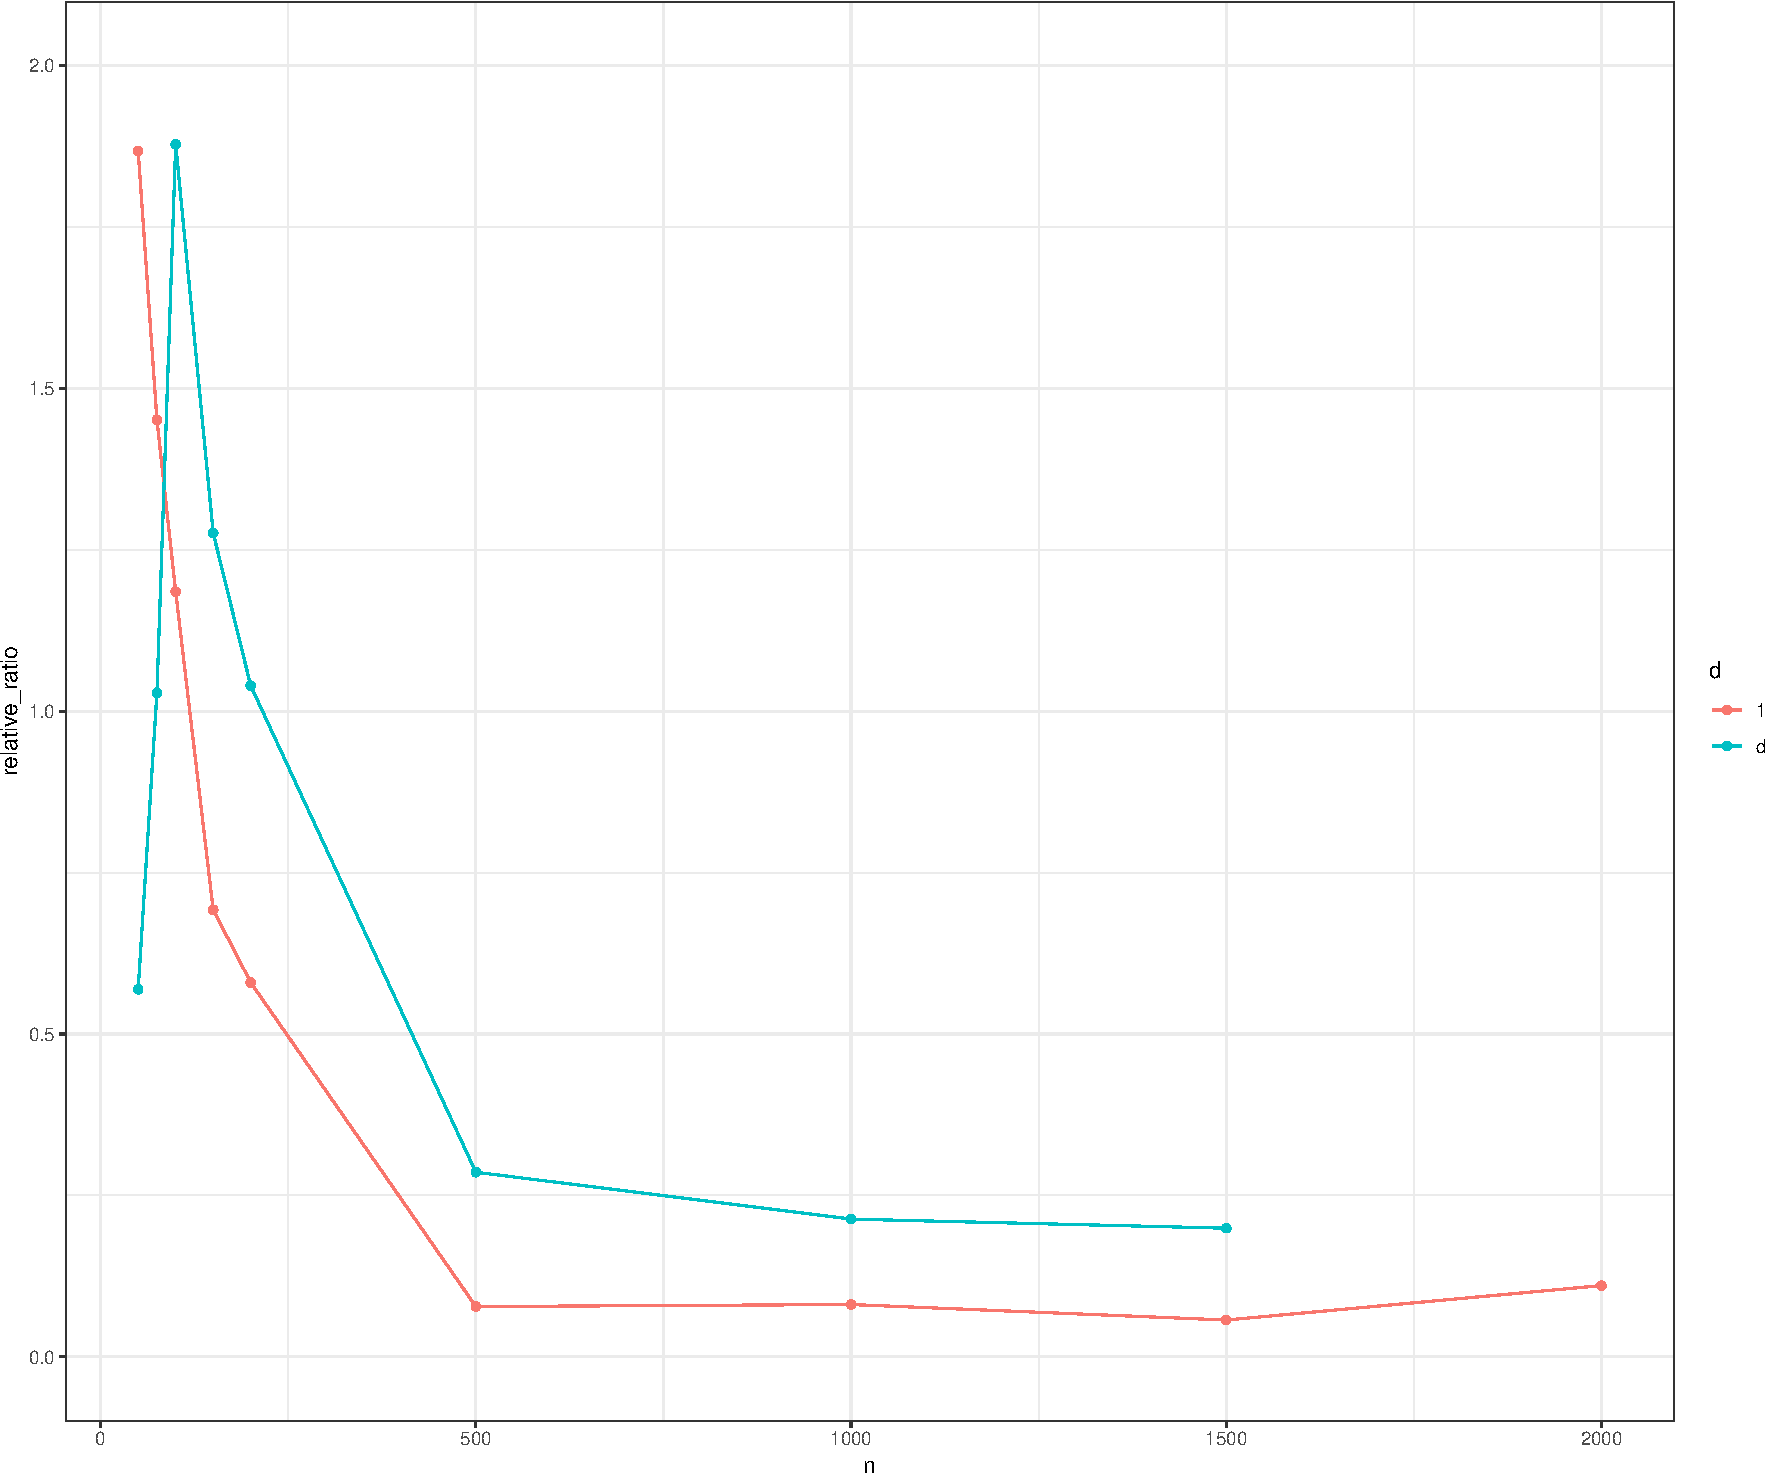
\includegraphics{GCTA_and_rr_v_jack_correction_iterations_files/figure-latex/unnamed-chunk-14-1.pdf}

\subsubsection{Eg with p = 100}\label{eg-with-p-100}

\begingroup\fontsize{5}{7}\selectfont

\begin{longtable}{rrrrrrrrrr}
\toprule
n & MSE & est\_var & est\_mean & NA\_main & EigenPrism\_main\_jack & EigenPrism\_v\_jack & EigenPrism\_v\_jack\_var & d & relative\_ratio\\
\midrule
\endfirsthead
\multicolumn{10}{@{}l}{\textit{(continued)}}\\
\toprule
n & MSE & est\_var & est\_mean & NA\_main & EigenPrism\_main\_jack & EigenPrism\_v\_jack & EigenPrism\_v\_jack\_var & d & relative\_ratio\\
\midrule
\endhead
\
\endfoot
\bottomrule
\endlastfoot
50 & 21.6516 & 21.7303 & 8.3722 & 0 & 7.6266 & 48.0986 & 454.15195 & 1 & 1.21343\\
50 & 21.6516 & 21.7303 & 8.3722 & 0 & -366.8806 & 48.3710 & 463.03961 & 25 & 1.22597\\
75 & 12.1880 & 12.2997 & 7.8937 & 0 & 7.3525 & 24.4991 & 94.99580 & 1 & 0.99184\\
75 & 12.1880 & 12.2997 & 7.8937 & 0 & -463.3255 & 25.6137 & 77.40674 & 38 & 1.08246\\
100 & 7.1233 & 7.1933 & 7.9561 & 0 & 7.0599 & 15.1132 & 40.83974 & 1 & 1.10102\\
\addlinespace
100 & 7.1233 & 7.1933 & 7.9561 & 0 & -710.8797 & 16.1844 & 33.40698 & 50 & 1.24993\\
150 & NaN & NA & NaN & 100 & NaN & NaN & NA & 1 & NaN\\
150 & NaN & NA & NaN & 100 & NaN & 8.4296 & 4.89393 & 75 & NA\\
200 & NaN & NA & NaN & 100 & NaN & NaN & NA & 1 & NaN\\
200 & NaN & NA & NaN & 100 & NaN & 5.0164 & 0.94967 & 100 & NA\\
\addlinespace
500 & NaN & NA & NaN & 100 & NaN & NaN & NA & 1 & NaN\\
500 & NaN & NA & NaN & 100 & NaN & NaN & NA & 250 & NaN\\
1000 & NaN & NA & NaN & 100 & NaN & NaN & NA & 1 & NaN\\
1000 & NaN & NA & NaN & 100 & NaN & NaN & NA & 500 & NaN\\
1500 & NaN & NA & NaN & 99 & NaN & NaN & NA & 1 & NaN\\
\addlinespace
1500 & NaN & NA & NaN & 69 & NaN & NaN & NA & 750 & NaN\\
2000 & NaN & NA & NaN & 100 & NaN & NaN & NA & 1 & NaN\\*
\end{longtable}

\endgroup{}

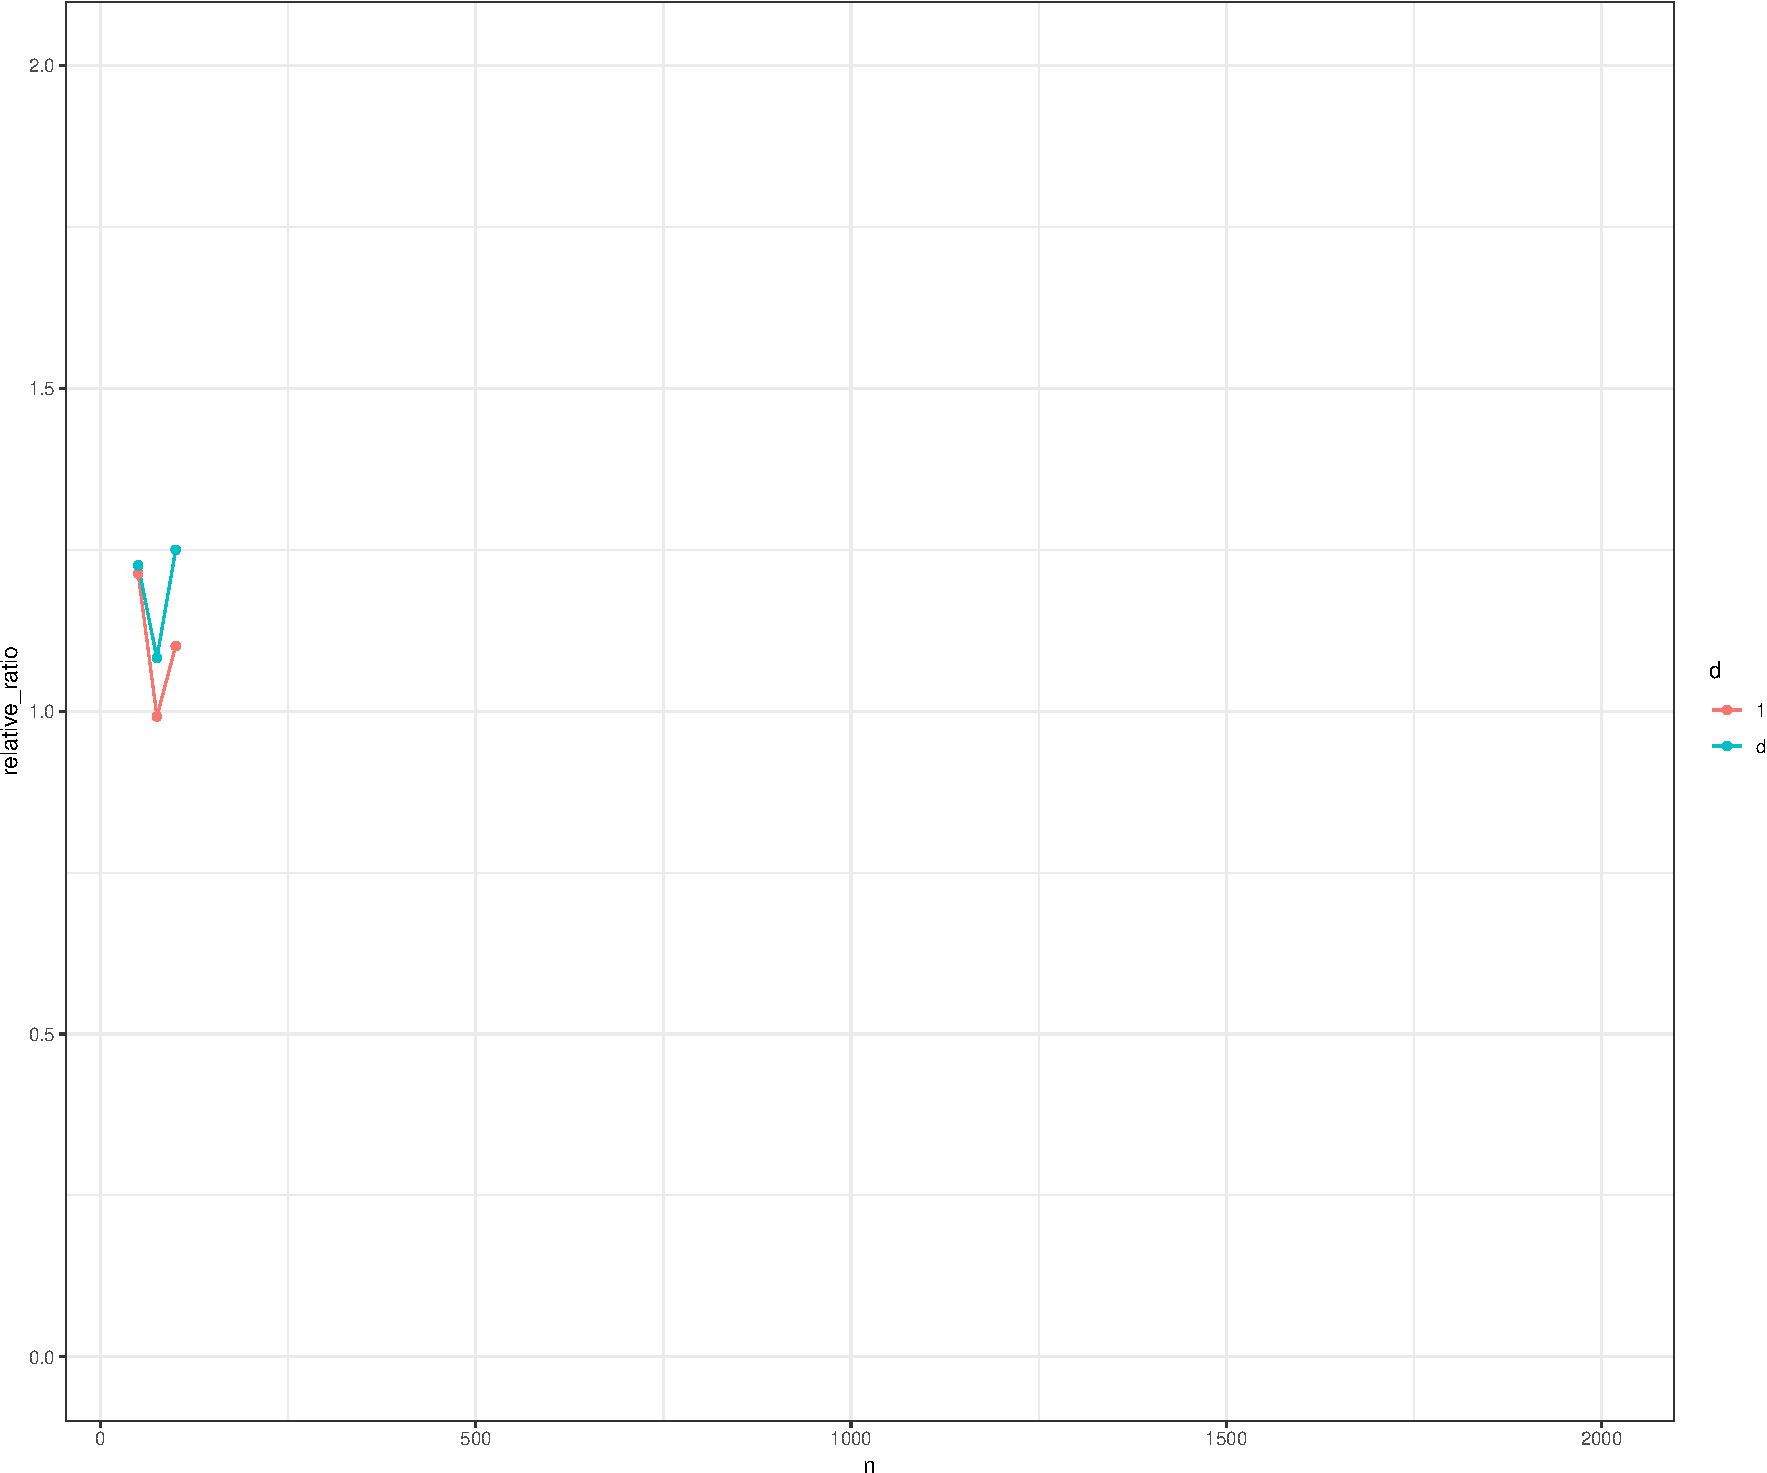
\includegraphics{GCTA_and_rr_v_jack_correction_iterations_files/figure-latex/unnamed-chunk-15-1.pdf}


\end{document}
